%!TEX root = ../Touch Based Idris.tex
\section{Second Design Iteration}
\label{sec:Implementation}

With an architecture in hand, it was time for the next design iteration.
As we mentioned in Section~\ref{subsec:first_design_evaluation}, several requirements and issues were still to resolved, and we felt the biggest remaining issue was the data declaration syntax.
It was the goal to create a prototype running on the iPad, ready for usability testing with a larger group of participants than in the mock-up phase.
Unfortunately, technical issues arose when implementing the many custom UI elements for the iPad prototype, which meant we had to be significantly less ambitious with regards to design changes from the first iteration.

\subsection{Data Declarations}
\label{subsec:second_data_declarations}
Our first priority was to improve the data declarations from our initial design. 
We followed \textbf{Re1} by splitting the name for the data and its type into two text fields, with a colon separating them. 
We also followed \textbf{Re2} by including text hints as to what should be in a text field.
These hints disappear as soon as the field gains focus.
The outlines around input fields were also changed to differentiate between fields that had been filled out, and fields that were yet to be filled out, as stated in \textbf{Re3}.
All these changes can be seen in Figure~\ref{fig:data_declaration}.

\begin{figure}
	\centering
		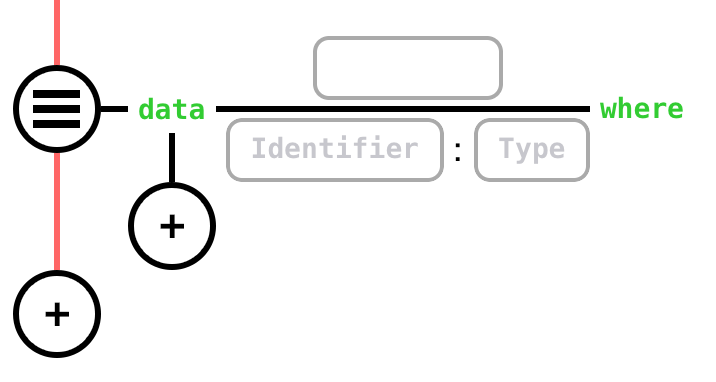
\includegraphics[width=70mm]{diagrams/data_declaration.png}
	\caption{A data declaration before the user has filled out anything.}
\label{fig:data_declaration}
\end{figure}

\subsection{Other Changes}
\label{subsec:other_changes}
Due to delays caused by the technical issues mentioned above, very few other changes, besides small tweaks, made it into this iteration.
In fact, one feature that was present in the original design did not make it into the prototype app, the TouchDevelop-like focus shifting, where different top-level elements would be in focus at different times. In this prototype all elements are in focus all the time. This goes against \textbf{U-6} and \textbf{F-9}. 
The final design can be seen in Figure~\ref{fig:initialiPadInterface}.

\begin{figure}
	\centering
		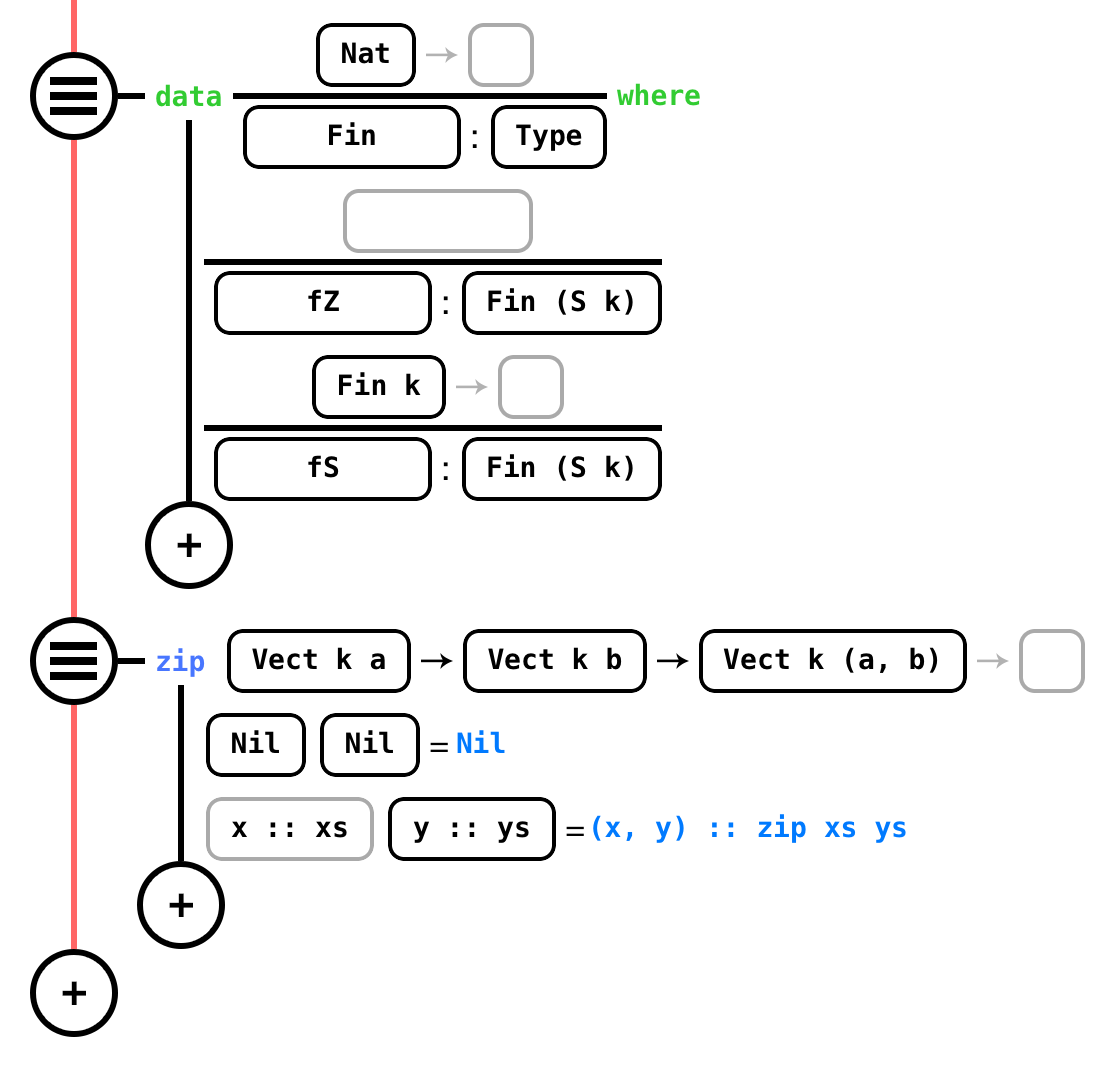
\includegraphics[width=110mm]{diagrams/ipad_interface.PNG}
	\caption{The initial iPad interface.}
\label{fig:initialiPadInterface}
\end{figure}

\subsection{Second Usability Iteration}
\label{sec:SecondUsabilityTest}
The greatest change in the second usability test was the fact that it was
performed on an actual iPad, using a prototype interface. The full report is
included in Appendix \todo{insert ref}. As in the first test, S2.4 refers to
the fourth point in the test summary for subject 2.

\subsubsection{Participants}
For our second usability test, we used two subjects from the first test,
subject \#1 and \#2. Their input was interesting, as they already had some
experience with the ideas in our representation from the mock-up test.
Hopefully this would let them focus more on the interactions with interface,
and less on learning a new way of presenting data. Subjects \#3 and \#4 had
never seen the interface before, and as such represented totally new users.
Their feedback was also very useful, as this iteration tried to make the first
time experience less frustrating.

\begin{table}[h]
\centering
\begin{tabular}{| l | l | p{5cm} | p{5cm} |}
\hline
Subject & Age & Occupation & Experience \\ \hline
\#1 & 24 & Masters student at IT-University studying programming languages & 7 months experience with Idris, several years of experience with functional languages in general \\ \hline
\#2 & 27 & Masters student at IT-University studying programming languages & 7 months experience with Idris, several years of experience with functional languages in general \\ \hline
\#3 & 27 & Masters student at IT-University studying programming languages & Very little experience with Idris. 1 year experience with Coq. Several years of experience with functional languages in general \\ \hline
\#4 & 23 & Masters student at IT-University studying programming languages & 6 months experience with Idris. Several years of experience with functional languages in general \\ \hline
\end{tabular}
\caption{Test subjects}
\label{table:second_test_subjects}
\end{table}

\subsubsection{Session Details}
Like the first test, this test was conducted in a meeting room at the IT
University, with three people present: The test subject, the test facilitator,
and a note taker. The tests were recorded. This time the test consisted of four
tasks, with the first task designed to get the subjects acquainted with the
data declarations, as per \textbf{Re4}. The next two tasks were identical to the first test, the
definition of the \texttt{Vect} data type and the \texttt{zip} function for
\texttt{Vect}. The final task concerned the manipulation of order of
declarations in the program they defined. As the app was still at prototype
stage, several bugs occurred during the subjects' use of the app. In these
cases the nature of the bug was quickly explained, and the facilitator
explained how to work around the issue.

\subsubsection{Tasks}
The four tasks they were asked to complete are listed in 
Figure~\ref{figure:second_tasks}.
As in the first test, the test subjects had access to the definitions for
\texttt{Vect} and \texttt{zip} textual Idris. See Section~\ref{subsec:Idris}
for more on \texttt{Vect} and \texttt{zip}.

\begin{figure}
\centering
\begin{itemize}
	\item \textbf{Task 1}: The user is shown the \texttt{Nat} and \texttt{Fin} data declaration in the program.
	\begin{itemize}
		\item \textbf{T1.1}: Describe the \texttt{Nat} type.
		\item \textbf{T2.2}: Describe the \texttt{Fin} type.
	\end{itemize}
	\item \textbf{Task 2}: Define a data declaration for the vector type.
	\begin{itemize}
		\item \textbf{T2.1}: Specify an identifier for the type (\texttt{Vect}), along with its type (\texttt{Nat -> Type -> Type})
		\item \textbf{T2.2}: Specify the Nil constructor (\texttt{Nil: Vect z a})
		\item \textbf{T2.3}: Specify the Cons constructor (\texttt{(::): a -> Vect k a -> Vect (S k) a})
	\end{itemize}
	\item \textbf{Task 3}: Define the zip function for vector type.
	\begin{itemize}
		\item \textbf{T3.1}: Specify the identifier for the function (\texttt{zip}), along with its type (\texttt{Vect k a -> Vect k b -> Vect k (a, b)})
		\item \textbf{T3.2}: Specify the first case (\texttt{zip Nil Nil = Nil})
		\item \textbf{T3.3}: Specify the second case (\texttt{zip x::xs y::s = (x, y) :: zip xs ys})
	\end{itemize}
	\item \textbf{Task 4}
	\begin{itemize}
		\item \textbf{T4.1}: Move the \texttt{Vect} declaration up below \texttt{Nat}.
	\end{itemize}
\end{itemize}
\caption{Tasks for the second usability test. The text in parentheses are what we considered the correct answer, and was not given to the test subjects.}
\label{figure:second_tasks}
\end{figure}

\subsubsection{Issues}
\label{sec:second_issues}
Many new issues were discovered in this usability test. This is not
surprising. In the first test, the facilitator took over the iPad's role, by
manipulating the mockups. This masked many flow and ease of use issues, which
have now been identified. During the test, several bugs were encountered. These
are not listed below, as they are not inherent to the design, but rather
results of the prototypical nature of the app.
\\ \\
\textbf{I5: Too many input fields}.
Most of the users reported that all the grey, unfilled input fields were
confusing. (S1.20, S2.2, S3.29b)
\todo{Insert screenshot}
\\ \\
\textbf{I6: Writing data declaration}
Everyone was able to decipher the data declarations almost immediately, but
all but one had trouble writing the \texttt{Vect} data declaration. Especially
the distinction between the premise area and the conclusion area seemed
problematic. (S1.1--1, S3.11--18, S4.3--7)
\\ \\
\textbf{I7: Arrows in data confusing}
The use of arrows in the premise area is confusing, as it implies a function. 
(S4.4)
\\ \\
\textbf{I8: Suggestions for parameterized types}
This issue persists from the original design. The subjects found it irritating
that after choosing a suggestion, they would have to manually change the
parameters using the standard iOS text editing facilities. Multiple subjects
mentioned that it broke their flow. (S1.10, S2.7, S3.15)
\\ \\
\textbf{I9: Lack of auto-closing parentheses and quotation marks}
We observed that users spent too much time navigating the virtual keyboards to
close pairs of symbols, when this can be done automatically.
\\ \\
\textbf{I10: Common symbols inaccessible}
In a similar vein, we noticed that some symbols commonly used when programming,
e.g. ``<'', took too long to find in the virtual keyboard.
\\ \\
\textbf{I11: Poor flow between input fields}
To move from one input field to the next, the subjects must manually tap each
input field. This broke the subjects flow. (S1.21, S3.30c)
\\ \\
\textbf{I12: Program can look cluttered}
After finishing all the tasks, the subject's program started to look cluttered.
\todo{Insert screenshot} (S3.29a)
\\ \\
\textbf{I13: Few definitions visible}
Related to Issue I12, definitions are quite large, so only a few are visible at
any time. This can make it hard for the subject to get an overview of their
work.
\\ \\
\textbf{I14: Unclear how to specify implicits and identifiers for arguments}
Some parts of the syntax have not been determined. Some of the subjects
wondered how one would make an argument implicit. (S1.9, S4.13)

\subsubsection{Recommendations}
\label{sec:second_recommendations}
As this represents the final iteration during this project, these
recommendations serve more as a reflection over how these issues might be
addressed.\todo{Ref to section with more reflection}

\begin{itemize}
    \item \textbf{Re8} (I5): Differentiate input fields to a greater degree. Perhaps outline required input fields in red, to differentiate them from other input fields.
    \item \textbf{Re9} (I5): Do not show input fields for declarations that do not have focus.
    \item \textbf{Re10} (I5): When centering text that includes an extra input field, center the text without the input field. \todo{Insert screenshot}
    \item \textbf{Re11} (I7): Use semicolons instead of arrows.
    \item \textbf{Re12} (I8): When showing types that take parameters, indicate these parameters in the popup. Then, after choosing one, create two new sub input fields, with their own suggestions. Make sure there is a good flow between these fields.
    \item \textbf{Re13} (I9): Automatically close pairs of symbols.
    \item \textbf{Re14} (I10): Include a shortcut bar for symbols.
    \item \textbf{Re15} (I11): After filling a field, automatically move input to next field. Perhaps include a button to move back and forth between fields.
    \item \textbf{Re16} (I12): Include more spacing between fields.
    \item \textbf{Re17} (I13): Include a cheat sheet on the right hand side, showing constructors and types for functions.
    \item \textbf{Re18}: In general, it might be good to separate text editing from general manipulation of the program. Text editing could occur in popups or a dedicated text input field, freeing gestures for other uses when manipulating the structure of the program.
\end{itemize}

\subsection{Design Evaluation}
\label{second_design_evaluation}
Unfortunately there were several recommendations from the first iteration that did not make it into this design. 
The missing functionality mentioned in Section~\ref{subsec:first_design_evaluation} also did not make it into this version.
While it is regrettable that we did not have a chance to test our recommendations or new features, the mere fact that we tested our design on an iPad led to a wealth of new insight.
We discovered many issues with the existing design that were only apparent when the design was put to use on a device. 
The final unmet usability requirement, to do with error handling (\textbf{U-6}), along with the functional requirements concerned with editing declarations (\textbf{F-4}, \textbf{F-5}) and quickly accessing special characters (\textbf{F-10}) will be addressed in the final design, presented in Section~\todo{ref}. 
This final design will also explore the recommendations from the first iteration (see Section~\ref{sec:first_recommendations}) that were not explored here, and experiment with a new way of declaring data.














